\documentclass{article}
\usepackage{ctex, hyperref}
\usepackage{graphicx}
\usepackage{amsmath}
\usepackage{hyperref}
\usepackage{amsfonts,amssymb}
\usepackage[top=2cm, bottom=2cm, left=2cm, right=2cm]{geometry}  
\usepackage{algorithm}  
\usepackage{algpseudocode}
\usepackage{float}  
\usepackage{listings} 
\title{作业二: 使用shell脚本实现对代码的测试}


\author{褚朱钇恒 \\ 信息与计算科学 3200104144}

\begin{document}

\maketitle

\section{使用背景}
    在写完一个程序后,我们可以用手动输入数据并肉眼观察输出的方法判断程序实现的正确性,但这种方法十分低效且有看错的可能,所以我们需要让计算机帮助我们实现这个步骤。

    我们可以准备一个保证正确的程序\verb|std.cpp|,和若干输入数据,以及一个需要判断正确性的程序\verb|NeedCheck.cpp|,然后让脚本实现编译两个程序,然后把数据一组一组分别喂给两个可执行文件,再比较两个输出是否相同。

\section{基本语法}
    \subsection{遍历输入文件}
        首先我们准备了24个输入文件,分别为\verb|01.in| $\cdots$ \verb|24.in|,然后在Beginning Linux Programming一书的第38页的\verb|Try It Out|中我们可以看到以下代码可以用于遍历所有带\verb|.sh|后缀名的文件
        \begin{verbatim}
#!/bin/sh
for file in $(ls f*.sh); do
lpr $file
done
exit 0
        \end{verbatim}

        那么我们稍加修改即可遍历所有输入数据
        \begin{verbatim}
#!/bin/sh
for file in $(ls *.in); do

done
exit 0
        \end{verbatim} 
    \subsection{比较文件内容}
        使用\verb|diff|命令即可比较文件内容,但两个程序输出的末尾可能有多余的空格或者换行,我们可以用\verb|-B|参数忽略文末换行,\verb|-b|参数忽略文末空格。

        如果\verb|diff|的两个文件相同,diff的返回值为真,否则为假,那么就可以根据\verb|diff|的返回值输出结果了。
    
    \subsection{输出各测试点结果}
        $\%$是去掉右边,\verb!${input_file%.*}!就可以给\verb|input_file|去掉后缀,只保留编号,那么我们就可以用以下代码输出结果表示该节点通过或没有通过测试。
        
        \begin{itemize}
            \item \verb|echo "Accept" ${input_file%.*}|
            \item \verb|echo "WrongAnswer" ${input_file%.*}|
        \end{itemize}

\section{实现}
    首先我们找两份代码\verb|std.cpp|和\verb|NeedCheck.cpp|,两者都来自同一道题目的提交记录,前者是我出题时写的正确代码,后者是比赛时某用户提交的错误代码。\href{https://ac.nowcoder.com/acm/contest/1115/C}{[牛客挑战赛33]艾伦的立体机动装置}

    然后我们找来构造的数据\verb|01.in| $\cdots$ \verb|24.in|。

    最后写出脚本代码\verb|run|

    (所有代码和数据都放在\verb|test|文件夹下)
\begin{verbatim}
#!/bin/bash
g++ std.cpp -o std
g++ NeedCheck.cpp -o wa
for input_file in $(ls *.in); do
	./std <$input_file >out1
	./wa <$input_file >out2
	if diff out1 out2 -b -B; then
		echo "Accept" ${input_file%.*}
	else 
		echo "WrongAnswer" ${input_file%.*}
	fi
done
\end{verbatim}

    接下来运行脚本就可以看到错误代码通过了哪些测试点,在哪些测试点输出了错误的答案。

    \begin{figure}[H]
        \centering
        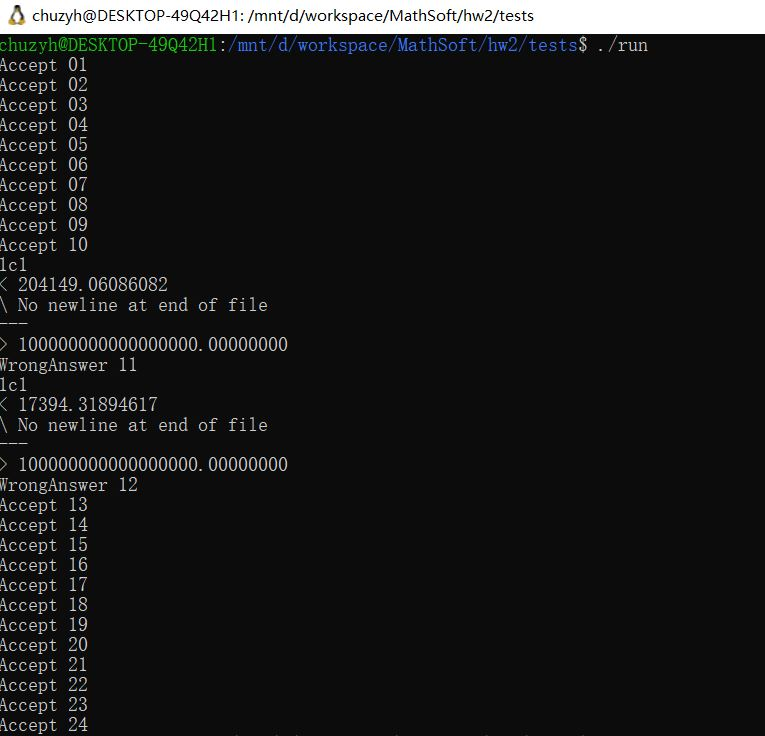
\includegraphics[scale=0.8]{result.JPG}
        \caption{运行结果}
      \end{figure}
\end{document}
